\section{Turbopompa}
\label{sec:turbopompa}

\subsection{Descrizione generica Mark 10}
\label{subsec:descrizione mark 10}

Il gruppo turbopompa Mark 10 è montato parallelamente alla mezzeria longitudinale della camera di spinta ed è sostenuto principalmente da due gruppi stabilizzatori a tre gambe saldati al corpo della camera e dai quattro condotti del propellente ad alta pressione installati tra la turbopompa e la camera di spinta. 
Il gruppo è composto da due pompe centrifughe montate schiena contro schiena (back-to-back) su un albero comune e azionate direttamente da una turbina a gas ad impulso.
L'albero principale e i componenti rotanti sono collegati direttamente all'albero e sono bilanciati dinamicamente.
L'albero è supportato da due gruppi di cuscinetti a sfere riscaldati elettricamente e raffreddati a carburante nell'area della pompa del LOX (per mantere l'ossigeno in fase liquid)e da un gruppo di cuscinetti a rulli raffreddati a carburante nell'area della turbina, mentre per isolare i propellenti, il fluido di raffreddamento e i gas caldi sono presenti un insieme di guarnizioni in carbonio, plastica (Kel-F, Teflon) e gomma sintetica (Buna-N, Viton-A).

\subsubsection{Pompe LOX e RP1}

L'esigenza di un sistema a turbopompa in uno stadio di lanciatore nasce quando il lanciatore stesso ha degli elevati requisiti di missione quali furono quelli dello stadio SI-C (e come la grande maggioranza dei primi e secondi stadi dei principali lanciatori odierni). Un sistema a serbatoio pressurizzato, per l'alimentazione dei 5 motori, dovrebbe essere progettato a sostenere elevate pressioni e quindi con un elevato spessore delle pareti dei tank. Introducendo il sistema di alimentazione a turbopompa, a patto di dimensionarlo correttamente, permette di diminuire il materiale per costruire i grandi tank di un sistema di queste dimensioni.
Tuttavia, un sistema cosi complesso introduce ulteriore complessità al progetto. Lo sviluppo moderno di tali sistemi prevede studi prelimiari con delle tecniche assodate da anni, come tabelle di valori specifici per le varie esigenze, con dati raccolti durante tutti gli anni di sviluppo.Al giorno d'oggi si conclude e si implementa la progettazione teorica tramite uno studio a CFD che tuttavia non verrà trattato in queste pagine. 

Entrando nel dettaglio del nostro sistema, entrambe le pompe del sistema Mark 10 sono di tipo centrifugo. Questo tipologia di pompa permette di avere un salto di pressione $\Delta P$ maggiore per singolo stadio rispetto alle pompe assiali, a discapito di un calo di efficienza. Questo trade-off permette di risparmiare in termini di peso e ingombro, a patto di contenere il decremento di efficienza con opportune scelte progettuali. Per pompe con fluido di lavoro a densità simile, come RP-1 e LOX, e simili pressione di scarico, si può mantenere la velocità angolare costante. 

%Un primo obiettivo nella progettazione della pompa è quello di %massimizzare la velocità operativa. In questo modo vengono %ridotte le dimensioni della stessa e di conseguenza il peso. Il %limite massimo giri al minuto non deve superare un limite %massimo per evitare cavitazione e sforzi centrifughi. 



\subsubsection{Analisi pompa LOX}
\rfig{OXIDIZER_PUMP}{Prospettiva e dettagli pompa LOX}{OXIDIZER_PUMP}{0.5}
Nei seguenti paragrafi verrà considerato il funzionamento a regime, in particolare si vuole proporre un'analisi della pompa LOX del sistema di interesse. Partendo da diverse ipotesi e alcuni dati trovati sui principali manuali di interesse (NASA design Criteria - TURBOPUMPS for LRE e Centrifugal pumps for LRE), verranno costruiti i triangoli di velocità di impeller e inducer. Si verificherà la loro sensatezza tramite un controllo in termini di salto entalpico prodotto. Nel processo di analisi si cercherà di dare una spiegazione dei vari componenti. Infine, tramite un programma MATLAB e la libreria CoolProp si cercherà di dare un'analisi più accurata producendo anche un diagramma dell'impeller del LOX e quindi avere un primo ingombro radiale. 

%METTERE LA TABELLA DEI DATI TROVATI 
METTERE IL PROCEDIMENTO DI RESH PER IMPELLER, INDUCER E DIFFSUER VANES SPIEGANDO LA FUNZIONE DI OGNI COMPONENTE E COME SI SONO RICAVATI I DATI 



%Il criterio principale da richiedere alla pompa è quello di avere una certa prevalenza, ovvero fornire un certo salto di pressione che viene calcolato in base ai requisiti di pressione  in camera e sommando le perdite lungo i collegamenti. Tale grandezza viene definita in termini di lunghezza o head-rise $H$ definito in questo modo
%\begin{empheq}{equation*}
%H = \frac{\Delta h_s}{g} = \int_{P_1}^{P_2} \frac{dp}{\rho g}
%\end{empheq}
%Dove $\Delta h_s$ è il salto entalpico del fluido che attraversa la pompa. La pompa deve anche fornire una certa portata richiesta, principalmente viene dettata dai requisiti in camera di combustione e gas generator, più eventuali perdite stimate. 
%A questi due requisiti sono solitamente associate due grandezze specifiche molto importanti in fase di progetto che sono $\psi$ ovvero l'head coefficient e $\phi$ il flow coefficient. Definiti in questo modo
%\begin{empheq}{gather}
%\phi = \frac{c_{m2}}{u_2}  \qquad \psi = \frac{\Delta H %g}{u_2 ^2 }
%\end{empheq}
%Dove $u_2$ è la velocità a diametro medio e velocità angolare di design, della paletta dell'impeller. Mentre $c_{m2}$ è la velocità merdionale, ovvero la componente della velocità assoluta che appartiene a piano radiale e assiale. 
%Un'altra grandezza specifica importante in fase di progetto è la velocità specifica $N_s$, definita in condizioni di design ovvero al numero di giri al minuto $N$ prestabiliti in condizioni stazionarie 
%\begin{empheq}{equation*}
%N_s = \frac{N\sqrt{Q}}{\Delta H^{0.75}}
%\end{empheq}
%Tale parametro permette di capire la tipologia di pompa su cui ci si deve concentrare per poter progettarla al meglio. Esso dipende da pochi fattori e come primo calcolo ci permette di capire quale impeller scegliere. Solitamente sono conosciuti i valori di portata e salto di pressioni richiesti, viene ipotizzato un numero di giri al minuto. 
%Durante il processo di design della pompa si deve considerare l'effetto della cavitazione presente all'inlet. Esso viene provocato per via di una depressione che si crea in ingresso alla pompa e deve essere agevolmente gestito per evitare danni catastrofici.  Per caratterizzare la condizione di cavitazione bisogna introdurre una nuova grandezza, detta NPSH (Net Positive Suction Head). In particolare:
%\begin{empheq}{equation*}
%\left(NPSH\right)_a = \frac{Pt - \Delta P}{\rho} - %P_{vap}
%\end{empheq}
%Tale grandezza indica la pressione in ingresso alla pompa. In fase di progettazione si utilizza il parametro $\left( NPSH \right)_c$ come pressione critica all'ingresso per non avere cavitazione. Si deve verificare che $\left( NPSH \right)_a > \left( NPSH \right)_c $.
%Per comparare le caratteristiche di aspirazione tra vari design di pompa centrifuga si utilizza un parametro simile alla velocità specifica, chiamato suction specific velocity $N_{ss}$ definito in questo modo.
%\begin{empheq}{equation*}
%N_{ss} = \frac{N\sqrt{Q}}{\left( NPSH \right)_c^{0.75}}
%\end{empheq}
%Alti valore di $N_{ss}$ (oltre i 50000) indicano la presenza di un inducer, a monte dell'impeller. Migliorando di fatto la prestazione della pompa. Si preferiscono valori alti di tale parametro perchè in tal modo si può aumentare il range di velocita rotazionali ammissibili dalla pompa senza incorrere in cavitazione, inoltre maggiorè è la velocità, minore sarà il peso totale della pompa. 

\subsection{Turbina}
\label{subsec:turbina}

\subsubsection{Descrizione turbina}

\rfig{turbina_general}{Turbina ad impulso VC dell'F-1}{turbina_general}{0.45}

La turbina che fornisce la potenza necessaria alle pompe del sistema motore F-1 è definita come turbina a impulso (variazione di pressione statica solamente negli statori), e cosiddetta 2 row - velocity compounded (VC). Ovvero costituita da 2 file di rotori intramezzati da uno statore. Il gas caldo prima di passare in questa zona viene espanso in una schiera di ugelli che aumentano notevolmente la velocità: per le turbina VC, idealmente, tutta l'espansione avviene in questa zona. Successivamente i rotori, venendo impattati da un gas, sottraggono quantità di moto al fluido. Lo statore intermedio ha la funzione di reinidirizzare il flusso all'ingresso dell'ultimo rotore. Oltre a queste zone citate, nella turbina c'è una zona di ingresso, manifold, che convoglia il flusso ai nozzles. I nozzles, che sono generalmente convergenti-divergenti per una turbina VC, espandono il gas e lo incurvano per affrontare il primo rotore. Entrambe le i rotori della turbina sono costituiti da dischi i quali presentano dei 'fir tree' slot lungo la circonferenza, dove vengono inserite e rivettate le palette. Il rotore iniziale è calettato direttamente sull'albero, l'ultimo viene imbullonato sul primo e vengono separati da un distanziale. Le guarnizioni sono di diverso tipo, in questa sede non verranno approfondite, ma hanno il compito di contenere le perdite e quindi migliorare l'efficienza. 

\subsubsection{Turbina - scelte progettuali}

Il sistema turbina di un endoreattore ha una vita breve ma è sottoposto a parecchi carichi critici. Il design deve essere compatto e leggero, il fluido che espande deve avere un alto contenuto energetico, il lavoro specifico in uscita deve essere alto. La progettazione dell'elemento turbina è direttamente collegato al tipo di ciclo di alimentazione del motore, nel caso di un GG si vuole massimizzare il salto di pressione per minimizzare la portata spillata prima della camera di spinta (questo infatti massimizza l'impulso specifico del sistema). 

Per l'analisi del percorso aerotermodinamico del gas si tratta un flusso di gas combusti a chimica congelata (FE). Tali parametri fisici sono stati interpolati tramite MATLAB da una tabella fornita dal libro [] (Modern engieering for LRE systems, AIAA, Huzel, ...), dati ricavati da test sperimentali di NASA. Di seguito vediamo quali parametri principali vengono utilizzati per la scelta e il dimensionamento della turbina. 

\begin{itemize}

\item
\textbf{Spouting velocity:} è la velocità teorica che il flusso di gas avrebbe se espandesse dalla pressione di ristagno alla pressione di uscita (data dal rapporto $\epsilon$ di espansione)
\begin{empheq}{gather*}
C_0 = \sqrt{2C_{p,gg}T_{in} \left(1 - \epsilon^\frac{1-\gamma }{\gamma}\right)}
\end{empheq}

\item
\textbf{Rapporto isoentropico delle velocità:} è il rapporto tra velocità tangenziale del disco rotorico e la spouting velocity.

\begin{empheq}{equation*}
\frac{U}{C_0} = 
\end{empheq}

\parbox[t]{\dimexpr\textwidth-\leftmargin}{%

\begin{wrapfigure}{r}{0.4\linewidth}
	\centering
	\vspace{-\baselineskip}
	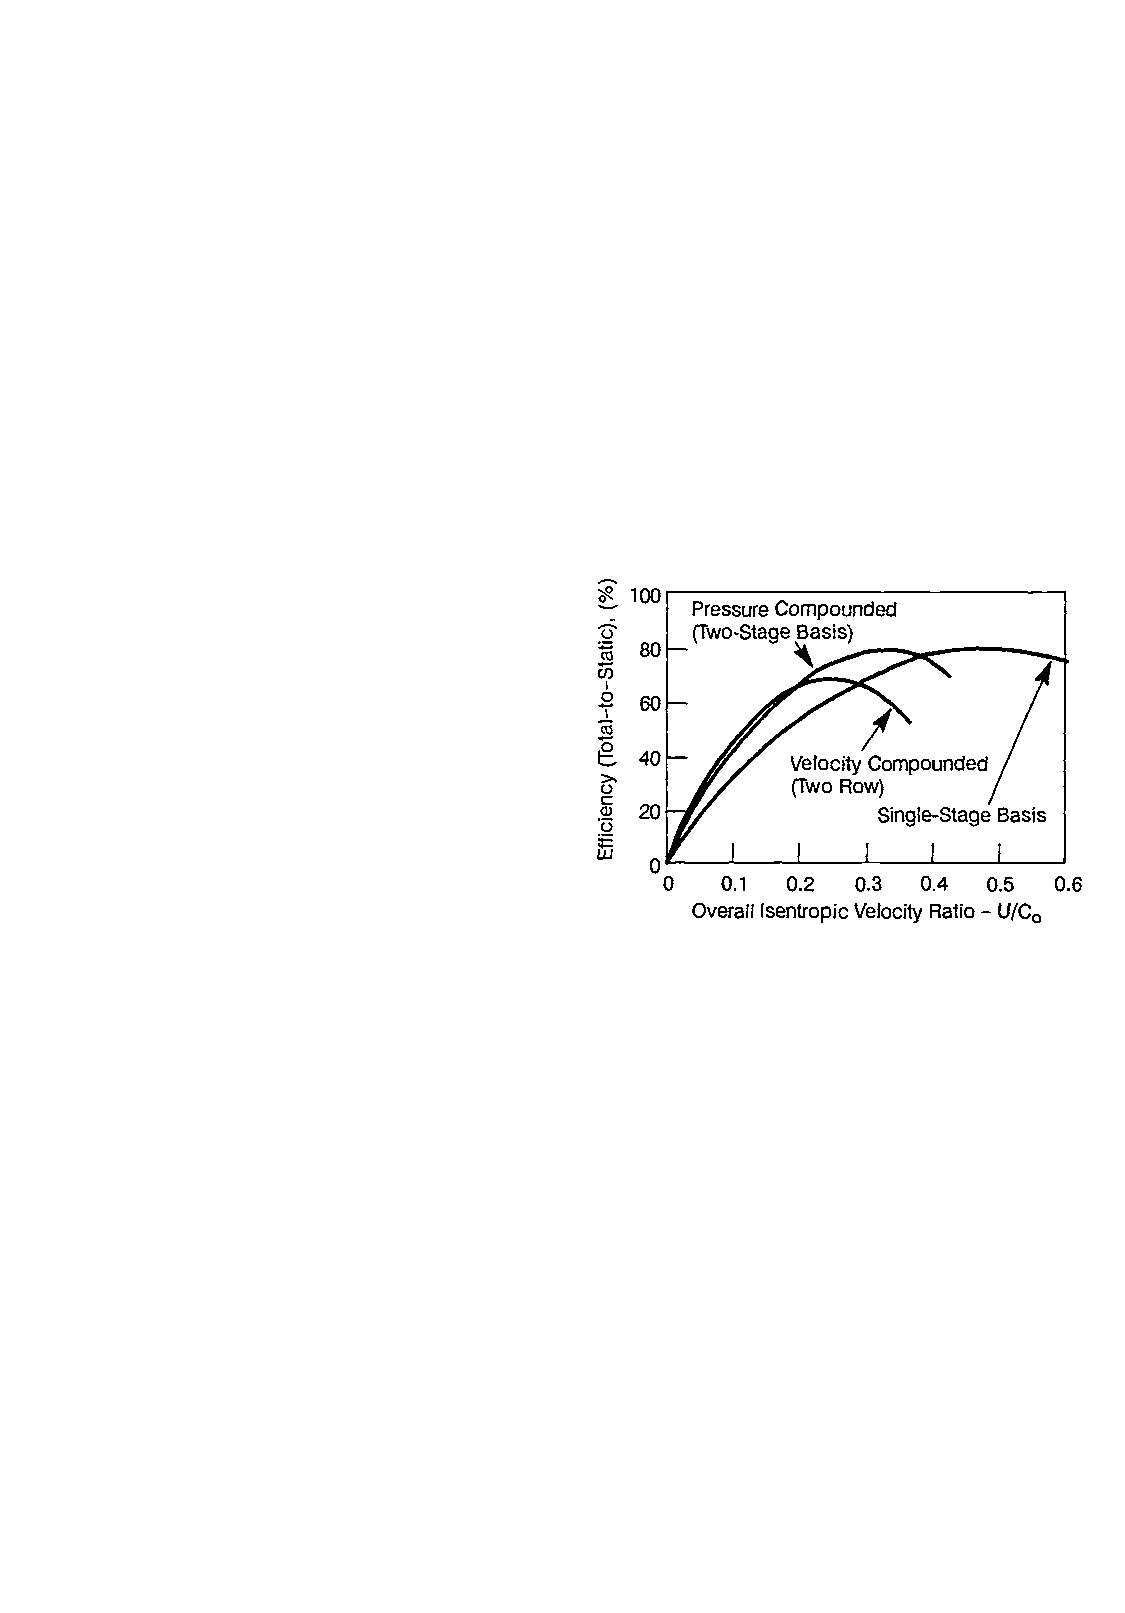
\includegraphics[width=\linewidth]{rendimenti_turbina}
	\caption{Rendimenti in funzione del rapporto di velocità}
	\label{fig:rendimenti_turbina}
\end{wrapfigure}

Questo valore è utile per capire la scelta progettuale effettuata per il tipo di turbina. Infatti, come già detto, nei cicli GG il salto di pressione in turbina è molto alto: questo implica un valore di $C_0$ elevato. Per avere una buona efficienza si possono percorrere più scelte progettuali (basandosi sul grafico x dei rendimenti). Si può scegliere di avere un alto rapporto di velocità con una singola ruota che 'assorba' tutta l'energia del flusso. Questo provocherebbe nel nostro caso una velocità di rotazione troppo elevata (quindi ingombro maggiore, inoltre la velocità di rotazione è fissata dalla pompa). Per usare altre turbine, cercando di avere un'alta efficienza si cerca di diminuire il rapporto di velocità aumentando gli stadi, ovvero la velocità del flusso è assorbita da più dischi che ruotano a velocità minori e sono più piccoli.

Le turbine PC (generano il salto di pressione in tutti gli statori) sono più efficienti ma più pesanti. Per cui si è optato per un sistema VC, che ha buona efficienza a bassi rapporti di velocità e permette un risparmio in peso.
}
\end{itemize}
\subsubsection{Analisi quantitativa - dimensionamento}

L'obiettivo ora è quello di cercare di dare un'idea a livello quantitativo dei vari componenti, generando un diagramma di velocità della turbina. 
Per questa sezione si sono presi in considerazione i requisti del sistema turbina, si sono ipotizzati diversi valori di rendimenti e sono state fatte alcune assunzioni ragionevoli per questo tipo di sistema (AIAA, modern engineering of LRE, Huzel ..). Abbiamo assunto i seguenti requisiti di sistema

\begin{table}[H]

\centering
\begin{tabular}{|c|c|c|c|c|c|}
\hline
$\bm{T_in \, [K]}$ & $\bm{p_in \, [bar]}$ & $\bm{\epsilon}$ &  $\bm{O/F}$ & $\bm{\dot{m} \, [kg/s]}$ & $\bm{\omega \, [rad/s]}$  \\
\hline
$1062$ & $67.57$ & $16.4$ &  $0.416$ & $75.75$ & $574.4$ \\
\hline
\end{tabular}

\caption{Requisiti del sistema turbina}
\label{table:turbine specs}

\end{table}

Assumendo tali dati, aggiungendo alcune ragionevoli ipotesi tratte dal libro AIAA e risolvendo il sistema di equazioni associato al problema, troviamo il seguente diagramma velocità e i corrispondenti valori di velocità e angoli. Si rimanda all'appendice per tutti i dettagli su ipotesi fatte, impostazione del sistema di equazioni e risoluzione del sistema tramite Matlab. 



